\chapter{Inclusione e taglio}


\section{Introduzione}

L'inclusione in paraffina è una fase fondamentale della preparazione istologica. Consiste nel lasciare permeare il tessuto da una sostanza solida a temperatura ambiente, in grado di supportare il taglio in sezioni sottili, solitamente dell'ordine di pochi micron. Questa sostanza è, nella pratica comune, la \textbf{paraffina}.


% Inserire figura 1: Immagine macro di un blocchetto di paraffina con tessuto incluso
 \begin{figure}[h]
 \centering
 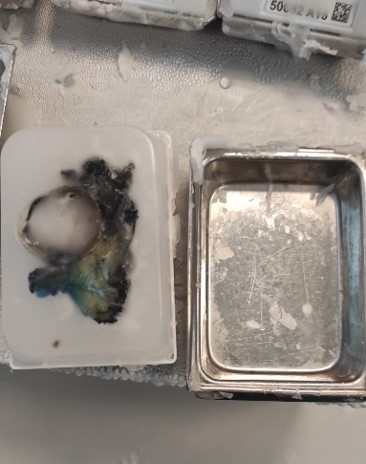
\includegraphics[width=0.5\textwidth]{inclusione_blocco_mold} 
 \caption{Blocchetto di paraffina con tessuto incluso.}
 \end{figure}

\section{La Processazione}

Prima dell'inclusione vera e propria, il tessuto deve essere sottoposto a un processo detto \textbf{processazione}, durante il quale viene progressivamente disidratato attraverso una scala alcolica crescente (dal 70\% al 100\%), quindi chiarificato con un intermedio come xilolo e infine infiltrato con paraffina calda (58–60 °C).

\section{Centralina di Inclusione}

La \textbf{centralina di inclusione} è lo strumento dove avviene il passaggio finale dell'infiltrazione: il campione viene posizionato in appositi stampi metallici (\textit{base molds}) e immerso nella paraffina fusa. Una volta orientato correttamente, il campione viene fatto solidificare.

% Inserire figura 3: Foto di una centralina di inclusione con operator* al lavoro
% \begin{figure}[h]
% \centering
% \includegraphics[width=0.6\textwidth]{centralina_inclusione.jpg}
% \caption{Centralina di inclusione in paraffina.}
% \end{figure}

\section{Criteri di Inclusione}

Un'inclusione corretta è essenziale per ottenere sezioni di qualità. I principali criteri da seguire sono:

\begin{itemize}
    \item Orientamento corretto del frammento.
    \item Scelta adeguata dello stampo.
    \item Assenza di bolle o crepe nella paraffina.
    \item Completa immersione del tessuto nella paraffina.
\end{itemize}

% Inserire figura 4: Immagine o disegno schematico di corretto orientamento
% \begin{figure}[h]
% \centering
% \includegraphics[width=0.5\textwidth]{orientamento_corretto.jpg}
% \caption{Esempi di orientamento corretto dei frammenti.}
% \end{figure}


\section{Inclusione in paraffina}

L'inclusione in paraffina è una fase fondamentale nella preparazione istologica, che consente il corretto sezionamento al microtomo. Il processo si svolge utilizzando una stazione di inclusione composta da tre elementi principali: la consolle termica, la consolle di dispensazione e la consolle criogenica.

\subsection{Panoramica dell'attrezzatura}

\begin{itemize}
  \item \textbf{Consolle termica}: mantiene i contenitori (mold o barchette) e le cassette di tessuto caldi dopo la processazione. Sono disponibili stampi di diverse dimensioni (piccolo, medio, grande). È consigliato mantenere questa zona pulita e asciutta.
  
  \item \textbf{Consolle di dispensazione}: contiene la paraffina fusa. Il serbatoio non deve essere riempito oltre i 3/4. Dispone di piastra calda, scalda-pinze e una leva per il rilascio della paraffina.

  \item \textbf{Consolle criogenica}: raffredda rapidamente i blocchi per solidificare la paraffina. Mantenere tra \(-4^\circ\)C e \(-7^\circ\)C. Accendere solo 20–30 minuti prima dell'uso per evitare danni.

  % FIGURA 1: Schema della stazione di inclusione
%   \begin{figure}[h!]
%     \centering
%     \includegraphics[width=0.85\textwidth]{embedding_station_overview.jpg}
%     \caption{Componenti principali della stazione di inclusione: consolle termica, di dispensazione e criogenica.}
%   \end{figure}

\end{itemize}

\subsection{Procedura di inclusione}

\begin{enumerate}
  \item \textbf{Preparazione}: accendere in anticipo la consolle termica e quella di dispensazione. Accendere la consolle criogenica la mattina stessa.

  \item \textbf{Gestione delle cassette}: aprire una sola cassetta per volta per evitare scambi accidentali di campione.

  \item \textbf{Scelta dello stampo}: selezionare la barchetta in base alla dimensione del campione. Campioni piccoli (testicoli, reni di topo) usano stampi piccoli; campioni grandi (es. fegato, cervello) richiedono stampi medi o grandi.

  \item \textbf{Incorporamento del tessuto}:
  \begin{enumerate}
    \item Aggiungere una piccola quantità di paraffina nella barchetta pre-riscaldata.
    \item Orientare il tessuto con pinzette calde, rispettando il protocollo del laboratorio (es. sezione sagittale o trasversale). Mantenere sempre la stessa direzione di orientamento.
    
    % % FIGURA 2: Orientamento corretto dei campioni
    % \begin{figure}[h!]
    %   \centering
    %   \includegraphics[width=0.75\textwidth]{sample_orientation.jpg}
    %   \caption{Esempi di orientamento corretto del tessuto per sezione sagittale e trasversale.}
    % \end{figure}
    
    \item Posizionare brevemente la barchetta sulla piastra fredda per fissare il campione con uno strato sottile di paraffina.
    \item Completare il riempimento della barchetta con paraffina, evitando la formazione di bolle (usare la croce sul coperchio per ridurle).
    \item Apporre il coperchio della cassetta e spostare la barchetta sulla consolle criogenica per il raffreddamento finale.
    

  \end{enumerate}
    % % FIGURA 3: Fasi dell'inclusione in paraffina
    % \begin{figure}[h!]
    %   \centering
    %   \includegraphics[width=0.85\textwidth]{embedding_steps.jpg}
    %   \caption{Fasi dell'inclusione in paraffina: versamento, orientamento, fissaggio, riempimento, raffreddamento.}
    % \end{figure}
  \item \textbf{Note operative}:
  \begin{itemize}
    \item \textbf{Pinzette}: alternare regolarmente tra pinzette calde per evitare che il campione si attacchi.
    \item \textbf{Raffreddamento rapido}: usare le zone più fredde per migliorare la cristallizzazione della paraffina e facilitare il sezionamento.
    \item \textbf{Campioni multipli}: allineare più campioni in una singola barchetta richiede velocità e precisione.
    


    \item \textbf{Uso di pesi}: appiattire campioni delicati (es. utero con ovaie) con pesi metallici appositi.
    \item \textbf{Posizionamento strategico}: posizionare il campione verso il basso della barchetta per facilitare il drenaggio durante la microtomia.
  \end{itemize}
\end{enumerate}
    % % FIGURA 4: Inclusione di campioni multipli
    % \begin{figure}[h!]
    %   \centering
    %   \includegraphics[width=0.75\textwidth]{multiple_embedding.jpg}
    %   \caption{Esempio di inclusione di campioni multipli in un unico blocco.}
    % \end{figure}
\subsection{Gestione dopo l'inclusione}

\begin{itemize}
  \item \textbf{Rimozione del blocco}: i blocchi devono staccarsi facilmente una volta completamente raffreddati. Se si oppongono resistenza, è segno che il raffreddamento non è stato sufficiente.
  
  \item \textbf{Controllo del livello}: i campioni devono essere incorporati sullo stesso piano. Eventuali dislivelli possono causare la perdita di sezioni durante il taglio.
  
  \item \textbf{Pulizia dei blocchi}: rimuovere la paraffina in eccesso dai bordi con un coltello smussato. Questo evita alterazioni dell'angolo di taglio al microtomo.
  
  \item \textbf{Conservazione}: se non si completa l’inclusione, avvolgere i campioni in carta stagnola e conservarli in modo ermetico. Evitare di lasciarli troppo a lungo nella zona calda.
\end{itemize}

\subsection{Pulizia e manutenzione}

Alla fine di ogni sessione:

\begin{itemize}
  \item Raschiare la paraffina residua da superfici e piastre con un coltello smussato.
  \item Svuotare il cassetto raccogli-paraffina.
  \item Riporre ordinatamente gli stampi per dimensione, facilitando il drenaggio e mantenendo l’area pulita.
\end{itemize}
 % FIGURA 5: Pulizia della stazione di inclusione
  %\begin{figure}[h!]
   % \centering
    %\includegraphics[width=0.75\textwidth]{cleaning_embedding_center.jpg}
    %\caption{Pulizia regolare della stazione di inclusione per garantire efficienza e sicurezza.}
  %\end{figure}
La pulizia regolare è essenziale per evitare accumuli, mantenere l'efficienza della stazione e garantire risultati riproducibili.



\subsection{Difetti Comuni nell'Inclusione}

\begin{itemize}
    \item \textbf{Crepe o bolle:} causate da raffreddamento troppo rapido o tessuti secchi.
    \item \textbf{Errata dispensazione della paraffina:} può causare spazi vuoti nel blocchetto.
    \item \textbf{Errore di orientamento:} compromette la leggibilità diagnostica.
    \item \textbf{Inquinamento da riporti:} contaminazione da tessuti diversi.
\end{itemize}

\section{Il Taglio al Microtomo}

Dopo l'inclusione, i blocchetti vengono tagliati con un \textbf{microtomo}. Le tipologie principali includono:

\begin{itemize}
    \item Microtomo rotativo (il più comune)
    \item Microtomo a slitta
\end{itemize}

\subsection{Fasi di Allestimento}

\begin{enumerate}
    \item Raffreddare i blocchetti su piastra refrigerata a –15/–5 °C.
    \item Pulire i blocchetti da eccessi di paraffina.
    \item Agganciare il blocchetto al porta blocco.
    \item Effettuare la sgrossatura.
    \item Tagliare sezioni dello spessore desiderato ($3–5\mu m$).
\end{enumerate}

% Inserire figura 5: Foto o illustrazione di un microtomo rotativo
% \begin{figure}[h]
% \centering
% \includegraphics[width=0.5\textwidth]{microtomo_rotativo.jpg}
% \caption{Microtomo rotativo per sezioni istologiche.}
% \end{figure}

\section{Caratteristiche di una Sezione Ottimale}

Una sezione ideale deve:

\begin{itemize}
    \item Essere ben centrata sul vetrino.
    \item Presentare spessore omogeneo.
    \item Essere priva di pieghe, strappi o bolle.
    \item Non presentare inquinamenti.
    \item Comprendere tutto il tessuto presente nel blocchetto.
\end{itemize}

\section{La tecnica di taglio}

Il microtomo è uno strumento progettato per ottenere sezioni sottili da campioni inclusi in paraffina, rendendoli idonei per la colorazione e l'osservazione microscopica. Di seguito si riassumono le principali operazioni da compiere per ottenere sezioni corrette.

\subsection{Fissaggio del blocchetto}

Utilizzare la leva dedicata per fissare saldamente il blocchetto al \textbf{porta-campione}. Questa operazione è fondamentale per garantire la stabilità durante il taglio.

% Inserire figura 7: Foto o disegno schematico del fissaggio del blocchetto nel porta-campione
% \begin{figure}[h]
% \centering
% \includegraphics[width=0.45\textwidth]{fissaggio_blocchetto.jpg}
% \caption{Fissaggio del blocchetto al microtomo.}
% \end{figure}

\subsection{Impostazione della lama}

La lama deve essere maneggiata con estrema attenzione. È buona norma sostituirla o regolarla prima del taglio di ogni nuovo campione. Il porta-lama è regolabile su tre piani mediante apposite manopole:

\begin{itemize}
    \item \textbf{Manopola anteriore}: regola l'inclinazione antero-posteriore.
    \item \textbf{Manopola sinistra}: consente l'allineamento laterale.
    \item \textbf{Manopola destra}: modifica l'angolo d'inclinazione.
\end{itemize}

In genere, si ottengono risultati ottimali con un'inclinazione piuttosto accentuata.

% Inserire figura 8: Schema delle tre manopole di regolazione del porta-lama
% \begin{figure}[h]
% \centering
% \includegraphics[width=0.55\textwidth]{regolazione_portalama.jpg}
% \caption{Regolazioni possibili del porta-lama.}
% \end{figure}

\subsection{Preparazione del blocchetto}

Prima del taglio vero e proprio, è necessario rimuovere lo strato esterno di paraffina per esporre il tessuto. Il blocchetto può essere immerso in acqua fredda per un periodo variabile da 1 a 24 ore per prevenire il distacco o lo “shattering” del tessuto durante il sezionamento.

Una volta esposto il tessuto, si può rifilare l'eccesso di paraffina con una lama da bisturi per ottimizzare la superficie da sezionare.

% Inserire figura 9: Immagine o illustrazione di rifilatura manuale del blocchetto
% \begin{figure}[h]
% \centering
% \includegraphics[width=0.5\textwidth]{rifilatura_blocchetto.jpg}
% \caption{Rifilatura della paraffina in eccesso.}
% \end{figure}

\subsection{Impostazione del microtomo}

Regolare lo spessore della sezione tramite l'apposita manopola (solitamente$3–5\mu m$). Utilizzare la ruota principale per avanzare il blocchetto contro la lama. Per motivi di sicurezza, il pomello laterale va abbassato e la manopola frontale estratta per attivare il movimento. Al termine dell'uso, riportare la manopola nella posizione iniziale.

% Inserire figura 10: Primo piano sul selettore dello spessore e sulla ruota del microtomo
% \begin{figure}[h]
% \centering
% \includegraphics[width=0.4\textwidth]{selettore_spessore.jpg}
% \caption{Regolazione dello spessore e controllo della ruota.}
% \end{figure}

\subsection{Raccolta delle sezioni}

Tagliare le sezioni in “nastri” di circa 6 sezioni ciascuno. Raccoglierli con pinzette e adagiarli delicatamente in un bagno d'acqua calda (45–50 °C) per distendere la paraffina. Con l'ausilio di un vetrino caricato (frosted side), raccogliere le sezioni e adagiarle su un nuovo vetrino portaoggetti.

% Inserire figura 11: Sequenza fotografica: taglio → raccolta → bagno caldo → vetrino
% \begin{figure}[h]
% \centering
% \includegraphics[width=\textwidth]{sequenza_raccolta.jpg}
% \caption{Sequenza di raccolta delle sezioni: dal taglio al vetrino.}
% \end{figure}

\subsection{Essiccazione}

Etichettare il vetrino con una matita indelebile e posizionarlo su una piastra riscaldante o in stufa a 37–40 °C per almeno un'ora, in modo da far aderire perfettamente le sezioni e rimuovere l'umidità residua.

% Inserire figura 12: Vetrini in essiccazione su stufa o piastra
% \begin{figure}[h]
% \centering
% \includegraphics[width=0.5\textwidth]{essiccazione_vetrini.jpg}
% \caption{Essiccazione dei vetrini prima della colorazione.}
% \end{figure}



\section{Difetti di Sezione e Correzioni}

\subsection{Effetto a Tapparella}

Linee parallele visibili nella sezione, spesso causate da disidratazione incompleta del tessuto.

\subsection{Pieghe}

Causate da compressione della sezione, dovuta a un blocco troppo caldo, lama non affilata o accumulo di cera.

\subsection{Bolle d'Aria}

Possono aderire sotto la sezione nel bagno d'acqua. Si consiglia di rimuovere bolle con un pennello prima di inserire la sezione.

\subsection{Crepe}

Si verificano con tessuti secchi o troppo processati. Visibili anche al microscopio dopo colorazione.

\subsection{Sezione Disintegrante}

Causata da tessuti poco infiltrati. Le sezioni assorbono acqua rapidamente e si disintegrano nel bagno caldo.

\textbf{Risoluzioni possibili:}
\begin{itemize}
    \item Aumentare lo spessore della sezione ($3–5\mu m$).
    \item Raffreddare meglio il blocchetto prima del taglio.
\end{itemize}

% Inserire figura 6: Serie di immagini di difetti di sezione (pieghe, crepe, tapparella)
% \begin{figure}[h]
% \centering
% \includegraphics[width=\textwidth]{difetti_sezione.jpg}
% \caption{Esempi di difetti comuni nelle sezioni istologiche.}
% \end{figure}

\section{Conclusioni}

L'inclusione in paraffina rappresenta una delle fasi più critiche nella preparazione di campioni istologici. Una corretta processazione, insieme a un'accurata inclusione e sezionamento, garantisce campioni di alta qualità per una diagnosi istopatologica precisa e affidabile.

